\subsection{Parallel production}
If there are any free modules available that perform work required by your recipes, then it can often be advantages to parallelize certain parts of your configuration using these modules. In this section we will produce a rule for inserting in free modules in order to parallelize certain works. We begin by describing the some required sets.

First we describe the set of pairs, where the first element is a module in between the modules $s$ and $e$ and the second element is a free module that can do atleast the work that the first element is currently doing.
\[Map_{s, e} = \{(m, m')| m \in FM \land m' \in M_{s,e} \land m'.aW \subseteq m.mW\} \]


We then describe all sets of pairs that could be a possible parallel line for the modules between $s$ and $e$. Note that this set could be the empty set, as the modules needed for creating a possible line might not availabe in $FM$.
\[MapPaths_{s,e} = \{p \in {Map}_{s,e}^2 | (m,m') \in p \land (n,n') \in p \land |p| = |M_{s,e}| \land  \forall m': m' \neq n' \}\]

We define $s[1]$ as the operation that given a set of pairs $s$, gives the set of all the first elements of the pairs in $s$.
\[s[1] = \{m_1 | (m_1, m_2) \in s\}\]

Using this we define the set $P_{s,e}$ as $MapPaths_{s,e}$ but without the second element in each pair.

\[ P_{s,e} = \{p[1] | p \in MapPaths_{s,e}\}\]

We can then total order this $P_{s,e}$ using the relation $<_p$ which is defined as follows.

\[a <_{p} b = 
\left\{\begin{matrix}
tt \texttt{ if } x \prec y \land (x, a), (y, b) \in MapPaths_{s,e}\\
\texttt{else } ff
\end{matrix}\right.\]

Now that we have defined these sets we can now describe the rules for parallezing a line in a configuration. We begin with the base case, in which we parallelize everything inbetween two modules. A graphical representation of this can be seen in \cref{fig:para_se}. As shown by the figure, if we can find a $P_{s,e}$ we parallize it by connecting it with transport modules to $s$ and $e$. The order in which $P_{s,e}$ is placed is the total order $(P_{s,e},<_p)$. 

\begin{figure}[h]
\centering
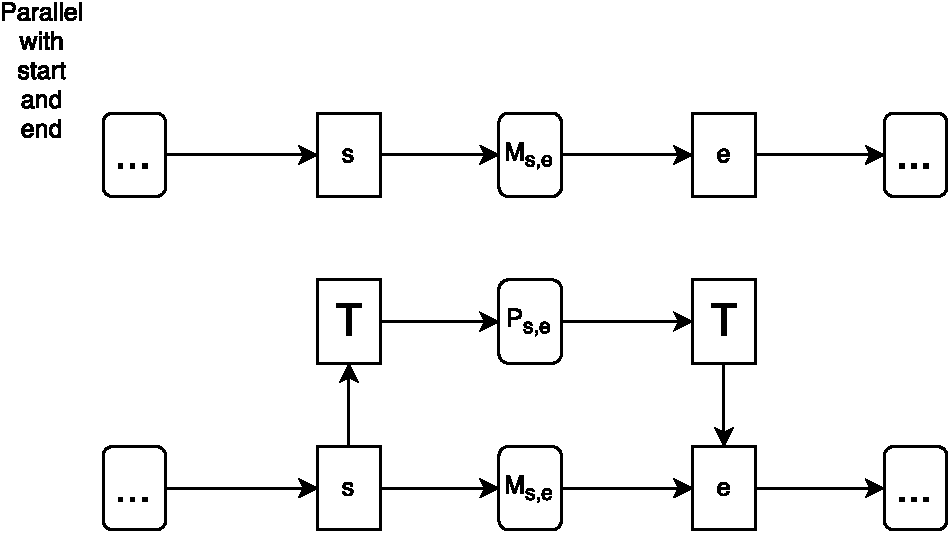
\includegraphics[width=0.5\textwidth]{para_se.pdf}
\caption{Parallelization rule when you have both a start and end module}
\label{fig:para_se}
\end{figure}


We also have two other cases, one in which we have no end module, meaning that we will fork out a parallel line, and the case where we have no start, meaning we will join in a parallel line. A graph showing both of these cases can be seen respectively in \cref{fig:para_we} and \cref{fig:para_ws}. For the case without start we connect the last module in the total order $(P_{s,e}, <_p)$ to $e$, and for the case without end we connect $s$ to the first module the in the total order $(P_{s,e}, <_p)$.


\begin{figure}[h]
\centering
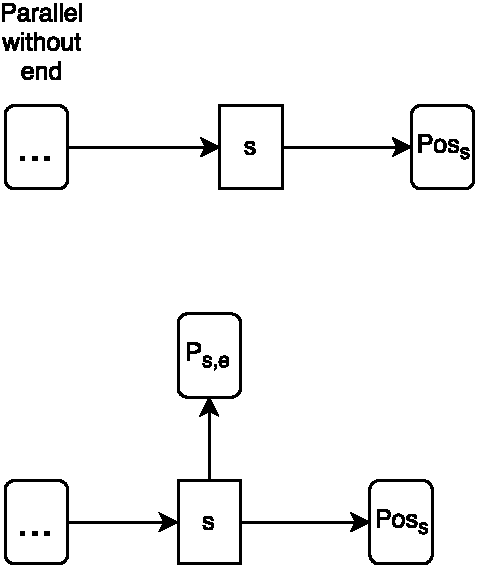
\includegraphics[width=0.3\textwidth]{para_we.pdf}
\caption{Parallelization rule when you do not have an end module}
\label{fig:para_we}
\end{figure}

\begin{figure}[h]
\centering
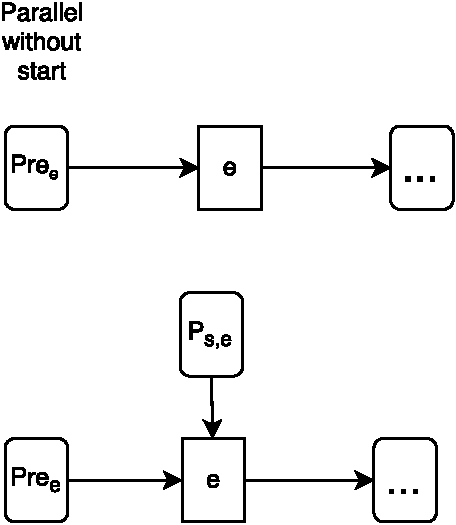
\includegraphics[width=0.3\textwidth]{para_ws.pdf}
\caption{Parallelization rule when you do not have a start module}
\label{fig:para_ws}
\end{figure}

